\documentclass{math}

\usepackage{forest}
\usepackage{listings}
\usepackage{tikz}
\usepackage{pgf-umlcd}
\usepackage{tikz-er2}
\usetikzlibrary{positioning}

\title{Principles of Data Management}
\author{Alvin Lin}
\date{August 2018 - December 2018}

\begin{document}

\maketitle

\section*{Database Interaction}
SQL alone is not enough to interact with a database. It cannot display a GUI
since it has no non-declarative actions. There are a few options:
\begin{itemize}
  \item Embedded SQL
  \item Dynamic SQL: ORM/interface
\end{itemize}
We can connect to a database via a direct connection, Open Database Connection
(ODBC), or Java Database Connection (JDBC). Both ODBC and JDBC add a level of
abstraction by acting as a proxy between the application and the database.
While it may slow things down by adding a layer of complexity, it allows you to
switch between databases seamlessly. The application developer can interface
with the ODBC/JDBC in a database agnostic manner. ODBC started out as a
Windows-specific platform but it has grown to almost every platform. Because
these interfaces cater to the lowest common denominator, they do not support
database-specific functionality and are primarily used for simple databases.

\subsection*{Interacting with Python (sample)}
\begin{lstlisting}[language=Python]
import psycopg2

conn_string = "host='reddwarf.cs.rit.edu'" \
              "dbname='db'" \
              "user='user'" \
              "password='pw'"
conn = psycopg2.connect(conn_string)
\end{lstlisting}
When connecting to a server, instead of copying data over the network
connection, it is usually always more efficient to use a server side cursor to
query the data. The server will instead hold a small portion of the database
in memory with the cursor pointing to the first element.
\begin{lstlisting}[language=Python]
cursor=conn.cursor()
cursor.execute("select * from car")
for data in cursor:
  print(data)
\end{lstlisting}

\subsection*{Database Design}
To reiterate, when planning the logical design of the database, we need to take
into account the business need of the database and the computer scientists who
need to build the application around the database.

\subsubsection*{Entity-Relationship Model}
\textbf{Entity}: anything that is distinguishable from other objects \\
\textbf{Entity Sets}: entities that are related (share some attributes)
\[ dog = (name,DOB,gooddog,breed,color,owner) \]
\begin{center}
  \begin{tabular}{|c|c|}
    \hline
    ID & Name \\
    \hline
    1 & Harry \\
    2 & Abbey \\
    3 & Potato \\
    4 & Kali \\
    5 & Sade \\
    \hline
  \end{tabular}
  \begin{tabular}{|c|c|}
    \hline
    ID & Name \\
    \hline
    1 & Jeff \\
    2 & Pat \\
    3 & Alvin \\
    4 & Andrew \\
    \hline
  \end{tabular}
\end{center}
\textbf{Relationship Sets}: links entity sets together
\begin{itemize}
  \item Harry - 2005 - Jeff
  \item Abbey - 2005 - Pat
  \item Potato - 2016 - Alvin
  \item Kali - 2018 - Andrew
  \item Sade - 2007 - Andrew
\end{itemize}
Binary relationships link two entities, but some relationships may have 3 or
more entities. Cardinality is used in binary degree relationship sets to define
how two entity sets are linked together.
\begin{itemize}
  \item One to One
  \item One to Many
  \item Many to One
  \item Many to Many
\end{itemize}

\subsection*{Complex Attributes}
Attributes can be simple or complex, single valued or multi-valued. Single
valued attributes are things like names, which we only have one of, while
emails are multi-valued since we can have multiple. Derived attributes are
things like age, which are derived from a date of birth. The domain of an
attribute is the set of available values for an attribute. Attributes like
names and addresses can be complex attributes:
\begin{center}
  \begin{forest}
    [name
      [given]
      [middle]
      [surname]
    ]
  \end{forest} \\
  \begin{forest}
    [address
      [street
        [number]
        [name]
        [apartment]
      ]
      [city]
      [state]
      [zip]
    ]
  \end{forest}
\end{center}

\subsection*{Redundant Attributes}
\[ cat=(name,owner.name,id,age) \]
\[ owner=(id,name,address) \]
The entities in weak entity sets are not unique.
\begin{center}
  \begin{tabular}{|c|}
    \hline
    Name \\
    \hline
    Andy \\
    Bob \\
    Andy \\
    Bob \\
    \hline
  \end{tabular}
\end{center}
Cat names in this example cannot uniquely identify a cat, so we link it to a
strong entity set, which contains an identifying entity. The weak entity set is
thus dependent on strong entity set. This provides a discriminating key or
attribute that can be added to the weak entity set to make it unique.

\subsection*{ER Diagrams}
Entity Set (UML and ER diagram):
\begin{center}
  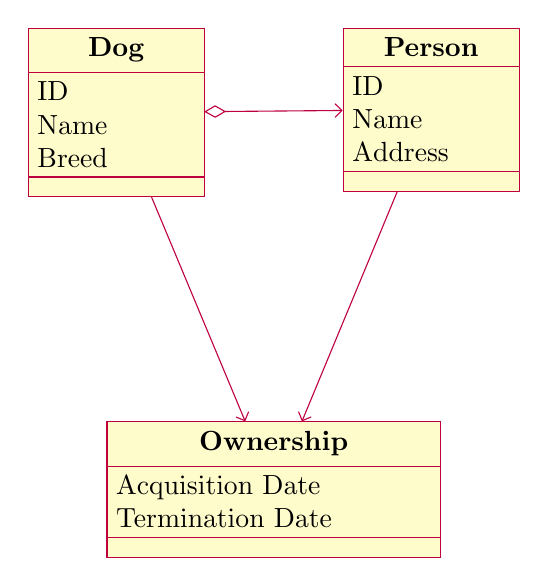
\begin{tikzpicture}
    \begin{class}[text width=2cm]{Dog}{0,0}
      \attribute{ID}
      \attribute{Name}
      \attribute{Breed}
    \end{class}
    \begin{class}[text width=2cm]{Person}{4,0}
      \attribute{ID}
      \attribute{Name}
      \attribute{Address}
    \end{class}
    \begin{class}[text width=4cm]{Ownership}{2,-5}
      \attribute{Acquisition Date}
      \attribute{Termination Date}
    \end{class}
    \aggregation{Dog}{}{}{Person}
    \unidirectionalAssociation{Dog}{}{}{Ownership}
    \unidirectionalAssociation{Person}{}{}{Ownership}
  \end{tikzpicture}
  \begin{tikzpicture}[node distance=0.5cm, every edge/.style={link}]
    \node[entity](dog){Dog};
    \node[attribute](dogname)[above left=of dog]{Name} edge (dog);
    \node[attribute](dogid)[above=of dog]{ID} edge (dog);
    \node[attribute](dogbreed)[above right=of dog]{Breed} edge (dog);

    \node[ident relationship](owns)[right=1.5cm of dog]{Owns} edge (dog);
    \node[attribute](ownsacquisition)[below left=1cm of owns]
      {Acquisition Date} edge (owns);
    \node[attribute](ownstermination)[below right=1cm of owns]
      {Termination Date} edge (owns);

    \node[entity](person)[right=5cm of dog]{Person} edge (owns);
    \node[attribute](personname)[above left=of person]{Name} edge (person);
    \node[attribute](personid)[above=of person]{Name} edge (person);
    \node[attribute](personaddress)[above right=of person]{Address} edge
      (person);
  \end{tikzpicture}
\end{center}
Dogs can also be related to other dogs, which can be represented as follows:
\begin{center}
  \begin{tikzpicture}[node distance=0.5cm, every edge/.style={link}]
    \node[entity](dog){Dog};
    \node[attribute](dogname)[above left=of dog]{Name} edge (dog);
    \node[attribute](dogid)[above=of dog]{ID} edge (dog);
    \node[attribute](dogbreed)[above right=of dog]{Breed} edge (dog);

    \node[ident relationship](owns)[right=3cm of dog]{Owns} edge[thick,double]
      node[above] {parent\_id} node[below] {pup\_id} (dog);
  \end{tikzpicture}
\end{center}

\subsubsection*{Cardinality}
\begin{itemize}
  \item 1:1
  \begin{center}
    \begin{tikzpicture}[node distance=0.5cm, every edge/.style={link}]
      \node[entity](dog){Dog};
      \node[entity](person)[right=6cm of dog]{Person};
      \node[ident relationship](owns)[right=2cm of dog]{Owns} edge[->] (dog)
        edge[->] (person);
    \end{tikzpicture}
  \end{center}
  \item Many:1
  \begin{center}
    \begin{tikzpicture}[node distance=0.5cm, every edge/.style={link}]
      \node[entity](dog){Dog};
      \node[entity](person)[right=6cm of dog]{Person};
      \node[ident relationship](owns)[right=2cm of dog]{Owns} edge[->] (dog)
        edge (person);
    \end{tikzpicture}
  \end{center}
  \item 1:Many
  \begin{center}
    \begin{tikzpicture}[node distance=0.5cm, every edge/.style={link}]
      \node[entity](dog){Dog};
      \node[entity](person)[right=6cm of dog]{Person};
      \node[ident relationship](owns)[right=2cm of dog]{Owns} edge (dog)
        edge[->] (person);
      \path (person) edge[bend right,->] node[above] {many} (dog);
      \path (dog) edge[bend right,->] node[below] {one} (person);
    \end{tikzpicture}
  \end{center}
\end{itemize}
A single line implies a 0..N relationship in that one thing can have 0 or more
of another object, while a double line implies 1..N which implies a one or more
relationship.

\subsubsection*{Complex Attributes}
UML:
\begin{center}
  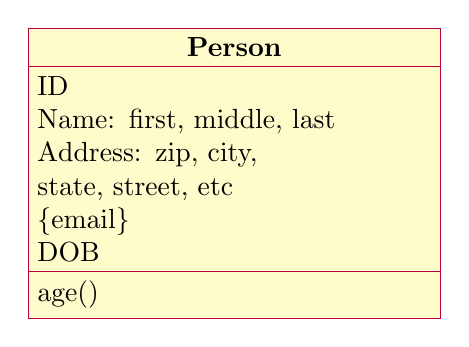
\begin{tikzpicture}
    \begin{class}[text width=5cm]{Person}{0,0}
      \attribute{ID}
      \attribute{Name: first, middle, last}
      \attribute{Address: zip, city, state, street, etc}
      \attribute{\{email\}}
      \operation{age()}
      \attribute{DOB}
    \end{class}
  \end{tikzpicture}
\end{center}
For the accompanying Chen ER diagram, multi-valued attributes like email are
double circled, while derived attributes like age are dotted.
\begin{center}
  \begin{tikzpicture}[node distance=0.5cm, every edge/.style={link}]
    \node[entity](person){Person};
    \node[attribute](id)[above=of person]{ID} edge (person);

    \node[attribute](name)[above right=of person]{Name} edge (person);
    \node[attribute](first)[above left=1cm of name]{First} edge (name);
    \node[attribute](middle)[above=of name]{Middle} edge (name);
    \node[attribute](last)[above right=1cm of name]{Last} edge (name);

    \node[attribute](address)[right=of person]{Address} edge (person);
    \node[attribute](zip)[above right=of address]{ZIP} edge (address);
    \node[attribute](street)[right=of address]{Street} edge (address);
    \node[attribute](number)[above right=of street]{Number} edge (street);
    \node[attribute](name)[right=of street]{Name} edge (street);
    \node[attribute](apartment)[below right=of street]{Apartment} edge (street);
    \node[attribute](etc)[below right=of address]{...} edge (address);

    \node[attribute,dotted](age)[below=1cm of person]{Age} edge (person);
    \node[attribute,double](email)[below left=of person]{Email} edge (person);
  \end{tikzpicture}
\end{center}
Sometimes, weak entity sets must rely on another entity in order to be uniquely
identified. For example:
\begin{center}
  \begin{tikzpicture}[node distance=0.5cm, every edge/.style={link}]
    \node[entity](employee){Employee};
    \node[attribute](id)[below=of employee]{ID} edge (employee);

    \node[ident relationship](hasa)[right=of employee]{Has A} edge (employee);

    \node[entity,double](child)[right=of hasa]{Child} edge[total] (hasa);
    \node[attribute,dotted](name)[above right=of child]{Name} edge (child);
    \node[attribute,dotted](dob)[below right=of child]{DOB} edge (child);
  \end{tikzpicture}
\end{center}
If there are two children (of two employees) with the same name and date of
birth, then they are reliant on their relationship with the employee and the
employee's ID in order to be uniquely identified.

\begin{center}
  You can find all my notes at \url{http://omgimanerd.tech/notes}. If you have
  any questions, comments, or concerns, please contact me at
  alvin@omgimanerd.tech
\end{center}

\end{document}
